\documentclass[11pt]{article}
%Gummi|061|=)
\usepackage{amsmath}
\usepackage{amsthm}
\usepackage{amsbsy}
\usepackage{amssymb}
\usepackage{inputenc}
\usepackage{graphicx}
\usepackage{selinput}
\SelectInputMappings{%
adieresis={ä},
germandbls={ß},
}
\title{\textbf{Versuch 303: Der Lock-In-Verstärker}}
\author{Martin Bieker\\
		Julian Surmann\\
		\\
		Durchgef\"{u}hrt am 05.12.2013\\
		TU
		 Dortmund}
\date{}
\usepackage{graphicx}
\begin{document}
\renewcommand\tablename{Tabelle}
\renewcommand\figurename{Abbildung}
\maketitle
\thispagestyle{empty}
\newpage
\clearpage
\setcounter{page}{1}


\section{Einleitung}
Im folgenden Versuch soll der Lock-In-Verstärker kennengelernt werden. Beim Lock-In-Verstärker handelt es sich um eine Schaltung, die ein stark verrauschtes Signal messbar macht.
\section{Theorie}
Um sehr schwache elektrische Signale zu messen, hat der Lock-In-Verstärker einen integrierten phasenempfindlichen Detektor. Zur Messung wird ein Signal mit einer beliebigen, aber konstanten Referenzfrequenz $w_0$ moduliert. Dieses Signal durchläuft den Messaufbau und wird dann mit einem geeigneten Empfänger wieder aufgenommen. Das aufgenommene Signal kann jetzt stark verrauscht sein, z.B. durch elektromagnetische Störquellen. Dieses Signal wird zunächst in einen Bandpass gespeist, sodass Störungen mit einer deutlich größeren $(w \gg w_0)$ bzw. kleineren Frequenz $(w \ll w_0)$ entfernt werden. Anschließend wird das Signal mit einem parallel erzeugten Referenzsignal der gleichen Frequenz im Mischer multipliziert. Die Phasenverschiebung zwischen den beiden Signalen ist dabei einstellbar, so können die Signale immer gleichphasig $(\Delta \phi) $eingestellt werden. Das bei der Multiplikation entstehende Signal wird schließlich in einen Tiefpass-Filter geführt. Dieser integriert das Signal über mehrere Perioden, sodass alle Störungen und das Rauschen fast restlos entfernt werden. Am Ausgang des Lock-In-Verstärkers liegt dann eine Spannung $U_{Out}$ an, die proportional ist zu der Spannung des Messsignals $U_{Sig}$. Indem man die Zeit der Integration $\tau = RC$ sehr groß wählt, kann man die Bandbreite des Rauschens $\Delta v = 1 / \pi RC$ beliebig verkleinern.\newline
Bei der Ausgangsspannung handelt es sich dann um die zur Signalspannung proportionale Spannung
\begin{equation}
U_{Out} = \frac{2U_0}{\pi}.
\end{equation}
Bei einer Phasendifferenz $\phi \neq 0$ gilt
\begin{equation}
U_{Out} = \frac{2U_0}{\pi}cos(\phi).
\end{equation}
\section{Aufbau und Durchf\"{u}hrung}
Zur Versuchsdurchführung steht ein modular aufgebauter Lock-In-Verstärker, ein digitales Speicheroszilloskop, eine Led und ein Photodetektor zur Verfügung. Es sollen insgesamt drei Messreihen durchgeführt werden.
Ein schematischer Aufbau ist der Abbildung ??? zu entnehmen.\newline
BILD\newline
Der Lock-In-Verstärker besteht aus einem Frequenzgenerator, einem Verstärker, einem Bandpass-Filter, einem Mischer und einem Lowpass-Filter mit integrierter variabler Verstärkung. Zusätzlich stellt das Modul einen Rauschgenerator zur Verfügung, um Störungen einer Messung zu simulieren. Ein digitales Speicheroszilloskop wird verwendet, um die Signale an verschiedenen Stellen des Signalwegs anzuzeigen und graphisch zu speichern. In den ersten beiden Messreihen wird die Schaltung je schrittweise aufgebaut, die Erste ohne und die Zweite mit Rauschgenerator. An dem Ausgang jedes verwendeten Bauteils wird dann das Ausgangssignal mit dem Oszilloskop graphisch aufgenommen.\newline
Im dritten Versuchsteil soll mit dem Frequenzgenerator eine Led periodisch zum Leuchten gebracht werden (BILD ???). \newline
\newline
Das Lichtsignal der Led wird dann mit einem in variabler Entfernung angebrachten Photodetektor erfasst und dann in den Verstärker gespeist. Das Signal ist jetzt durch das Umgebungslicht verrauscht, der eingebaute Rauschgenerator wird also nicht verwendet. Der Phototransistor wird immer weiter von der Led entfernt und die Ausgangsspannung des Lowpass-Filters ermittelt, um eine Aussage darüber zu treffen, bis zu welcher Entfernung das Signal der Led noch nennenswert erfasst wird.
\section{Auswertung}
\subsection{Aufbau und Auswertung der Schaltungen 1.A und 1.B}
\subsubsection{Funktionengenerator}
Der Funktionengenerator erzeugt zwei Signale, die an separaten Ausgängen anliegen. Am linken Ausgang liegt das Messsignal an, bei dem es sich um eine Rechteck- oder Sinusspannung handelt. Der rechte Ausgang ist für das Referenzsignal bestimmt. Die Amplitude des rechten Ausgangs liegt konstant bei ??? V. Am linken Ausgang liegt eine eingestellte Spannung von $10 \, mV$ bei einer Frequenz von $1000 \, Hz$ an. Das mit dem Oszilloskop gemessene Signal ist in Abbildung ??? zu sehen.
\subsubsection{Rauschgenerator (Nur 1.B)}
Der Rauschgenerator wird nur in Schaltung 1.B eingesetzt. Er addiert ein Rauschen auf das Signal. Dies ist in Abbildung ??? zu sehen. 
\subsubsection{Vorverstärker}
Der Vorverstärker verstärkt das Signal (Abbildungen ??? und ???). Bei beiden Signalen ist zu sehen, dass sich lediglich die Amplitude der Signale ändert.
\subsubsection{Bandpass-Filter}
Der Bandpass-Filter wird auf die Frequenz des Funktionengenerators eingestellt. Damit werden grob die Anteile des Rauschens entfernt, deren Frequenz deutlich von der des Messsignals abweicht (Abbildungen ??? und ???). An dem unverrauschten Signal ändert sich nichts, bei dem Verrauschten Signal wird ein Teil des Rauschens bereits entfernt.
\subsubsection{Mischer}
Der Mischer addiert das Messsignal und das Referenzsignal miteinander (Abbildungen ??? und ???). Durch diese Mischung wird eine Gleichrichtung erzeugt, diese ist deutlich zu erkennen.
\subsubsection{Lowpass-Filter}
Der Lowpass-Filter mit dem Integrierglied integriert das Signal über mehrere Perioden des Signals. Dadurch werden die meisten Rauschsignale entfernt. Die mittlere Ausgangsspannung wird für verschiedene Phasenverschiebungen mit Hilfe eines Voltmeters gemessen. Die Messwerte sind den Tabellen ??? und ??? zu entnehmen.

\section{Diskussion}
Hier kommt die Diskussion hin.
\section{Literatur- und Abbildungsverzeichnis}
Hier befindet sich das Literatur- und Abbildungsverzeichnis.


\section{Anhang}
\begin{itemize}
\item Tabelle 1: $U_{out}$ in Abhängigkeit von $\Delta\phi$ (unverrauschtes Signal)
\item Tabelle 2: $U_{out}$ in Abhängigkeit von $\Delta\phi$ (verrauschtes Signal)
\item Tabelle 3: Messergebnisse der Photodetektorschaltung
\item Abbildungen \ref{Abb1} bis \ref{Abb14}: Mit dem Oszilloskop erstellte Screenshots
 
\end{itemize}
\newpage

\begin{table}[h!]
\centering
\begin{tabular}{|c|c|c|c|}
\hline
$\Delta \phi [^\circ]$ & $U_{out}^* [V]$ & Gain & $U_{out} [V]$ \\
\hline
0.0 & -5.3 & 2 & -2.65\\
30.0 & -4.8 & 2 &-2.4\\
60.0 & -1.9 & 2 &-0.95\\
90.0 & 0.0 & 2 &0.0\\
120.0 & 2.3 & 2 &1.15\\
150.0 & 4.9 & 2 &2.45\\
180.0 & 5.4 & 2 &2.7\\
210.0 & 4.9 & 2 &2.45\\
240.0 & 2.0 & 2 &1.0\\
270.0 & 0.1 & 2 &0.05\\
300.0 & -2.0 & 2 &-1.0\\
330.0 & -4.8 & 2 &-2.4\\
\hline
\end{tabular}
\label{data1}
\caption{Ausgangsspannung bei verschiedenen Phasenverschiebungen \newline (unverrauschtes Signal)}
\end{table}


\begin{table}[h!]
\centering
\begin{tabular}{|c|c|c|c|}
\hline
$\Delta \phi [^\circ]$ & $U_{out}^* [V]$ & Gain & $U_{out} [V]$ \\
\hline
0.0 & 5.0 & 10.0 & 0.5\\
30.0 & 4.5 & 10.0 & 0.45\\
60.0 & 2.1 & 10.0 & 0.21\\
90.0 & 0.5 & 10.0 & 0.05\\
120.0 & -1.7 & 10.0 & -0.17\\
150.0 & -3.8 & 10.0 & -0.38\\
180.0 & -4.2 & 10.0 & -0.42\\
210.0 & -3.8 & 10.0 & -0.38\\
240.0 & -1.4 & 10.0 & -0.14\\
270.0 & 0.4 & 10.0 & 0.04\\
300.0 & 2.3 & 10.0 & 0.23\\
330.0 & 4.6 & 10.0 & 0.46\\
360.0 & 5.0 & 10.0 & 0.5\\
\hline
\end{tabular}
\label{data2}
\caption{Ausgangsspannung bei verschiedenen Phasenverschiebungen \newline (verrauschtes Signal)}
\end{table}


\begin{table}[h!]
\centering
\begin{tabular}{|c|c|c|c|c|}
\hline
$d^* [m]$ & $d [m]$ & $U_{out}^*$ & Gain & $U_{out}$ \\
\hline
0.06 & 0.024 & 6.6 & 2.0 & 3.3\\
0.16 & 0.124 & 4.7 & 20.0 & 0.235\\
0.26 & 0.224 & 8.3 & 100.0 & 0.083\\
0.36 & 0.324 & 4.5 & 100.0 & 0.045\\
0.46 & 0.424 & 6.5 & 200.0 & 0.0325\\
0.56 & 0.524 & 5.1 & 200.0 & 0.0255\\
0.66 & 0.624 & 4.0 & 200.0 & 0.020\\
0.76 & 0.724 & 8.6 & 500.0 & 0.0172\\
0.86 & 0.824 & 7.9 & 500.0 & 0.0158\\
0.96 & 0.924 & 7.4 & 500.0 & 0.0148\\
1.06 & 1.024 & 6.9 & 500.0 & 0.0138\\
1.16 & 1.124 & 6.6 & 500.0 & 0.0132\\
1.26 & 1.224 & 6.5 & 500.0 & 0.0130\\
1.36 & 1.324 & 6.1 & 500.0 & 0.0122\\
\hline
\end{tabular}
\label{data}
\caption{Messergebnisse der Photodetektorschaltung}
\end{table}


\begin{figure}[h]
\centering
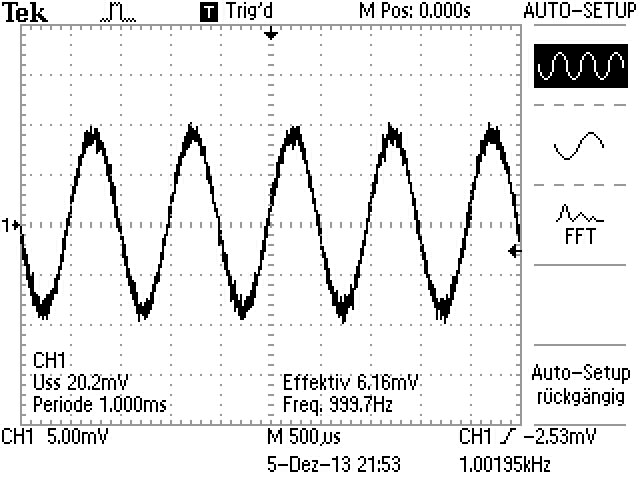
\includegraphics[scale=0.85]{Bilder/1-sine.png}
\caption{Signal vom Sinusgenerator}
\label{Abb1}
\end{figure}
\begin{figure}[h]
\centering
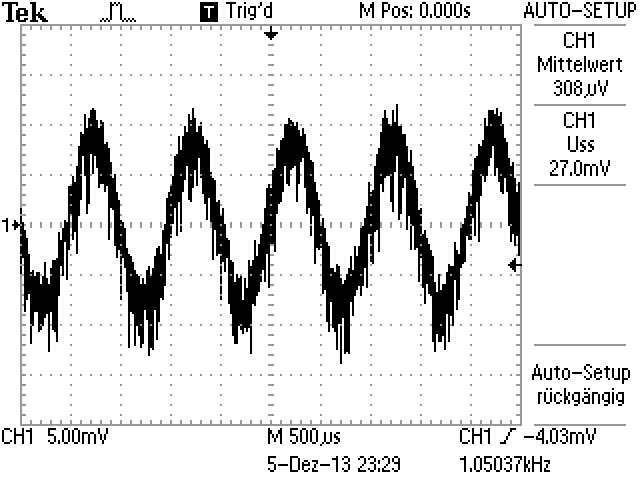
\includegraphics[scale=0.85]{Bilder/2-noise.png}
\caption{Unverstärktes Signal mit Rauschen}
\label{Abb2}
\end{figure}
\begin{figure}[h]
\centering
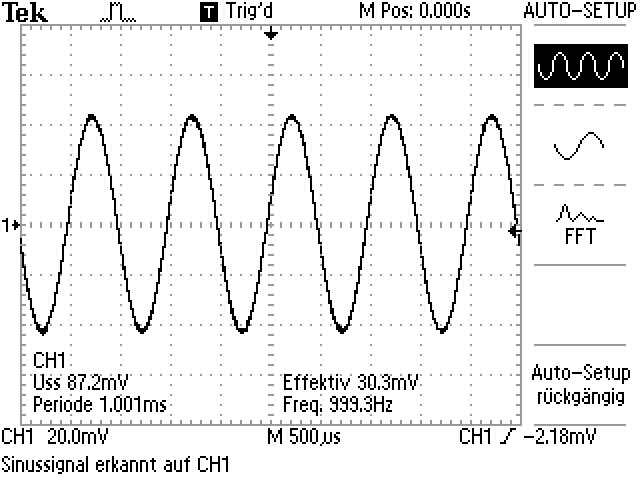
\includegraphics[scale=0.85]{Bilder/3-sine.png}
\caption{Verstärktes Signal ohne Rauschen}
\label{Abb3}
\end{figure}
\begin{figure}[h]
\centering
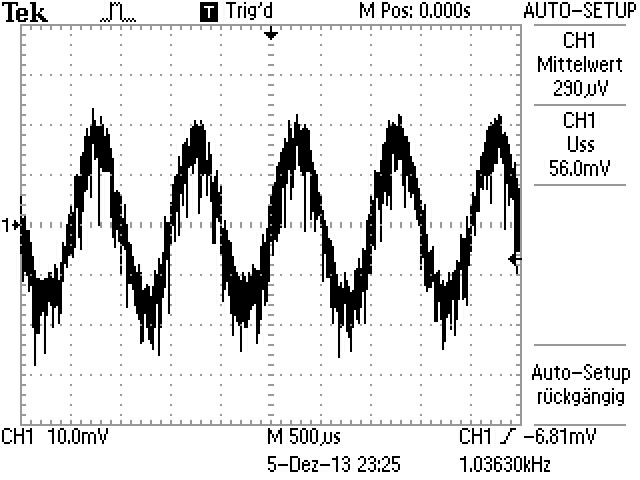
\includegraphics[scale=0.85]{Bilder/3-noise.png}
\caption{Verstärktes Signal mit Rauschen}
\label{Abb4}
\end{figure}
\begin{figure}[h]
\centering
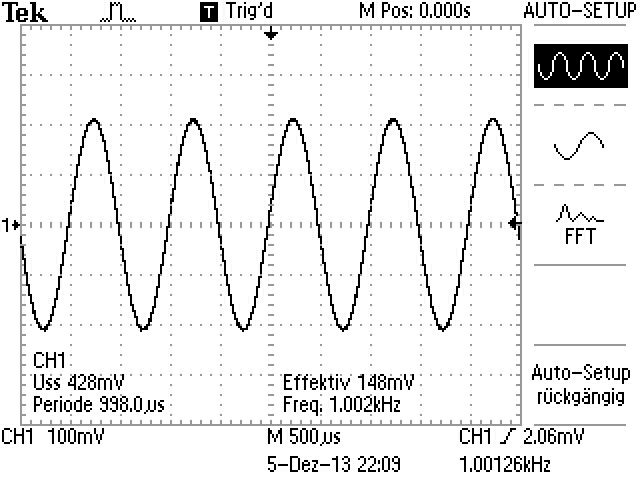
\includegraphics[scale=0.85]{Bilder/4-sine.png}
\caption{Output des Bandpassfilters }
\label{Abb5}
\end{figure}[h]
\begin{figure}
\centering
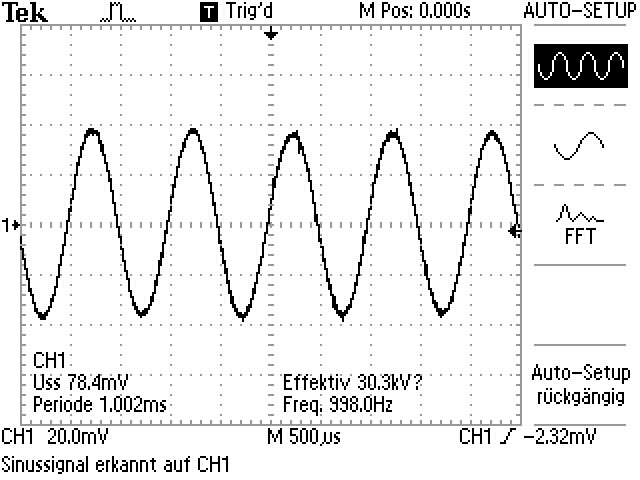
\includegraphics[scale=0.85]{Bilder/4-noise.png}
\caption{Output des Bandpassfilters (verrauscht)}
\label{Abb6}
\end{figure}

\begin{figure}[h]
\centering
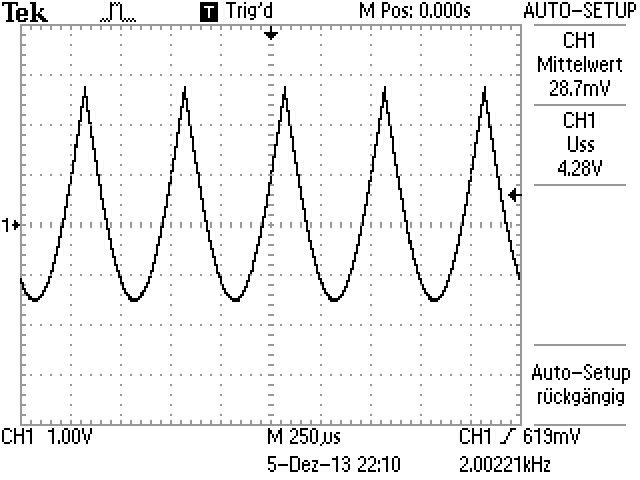
\includegraphics[scale=0.85]{Bilder/5-sine-0.png}
\caption{Output des Mischers bei unverrauschtem Signal ($\Delta\phi=0^\circ$)}
\label{Abb7}
\end{figure}

\begin{figure}[h]
\centering
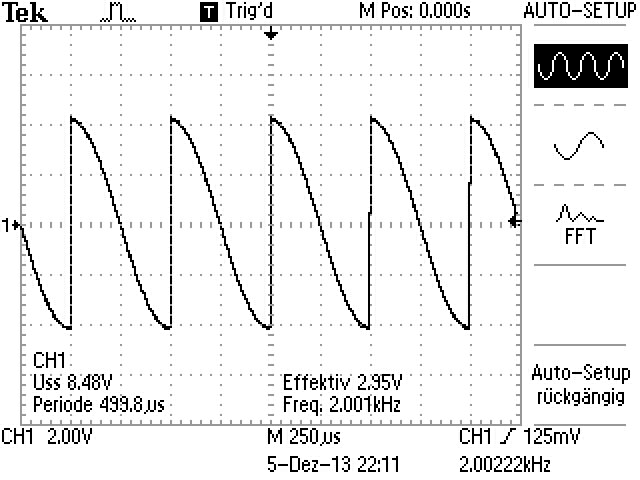
\includegraphics[scale=0.85]{Bilder/5-sine-90.png}
\caption{Output des Mischers bei unverrauschtem Signal ($\Delta\phi=90^\circ$) }
\label{Abb8}
\end{figure}

\begin{figure}[h]
\centering
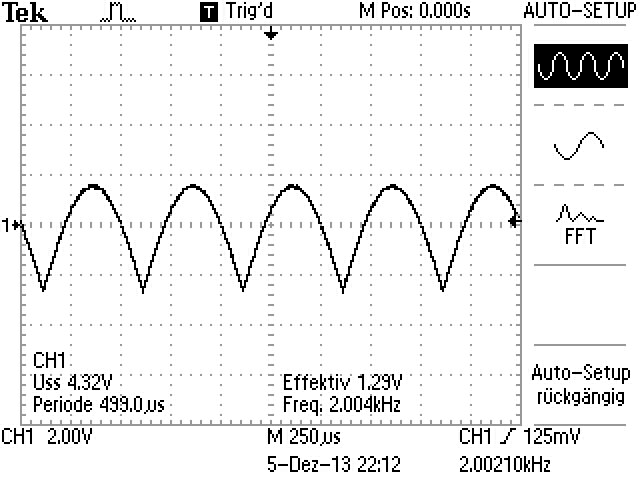
\includegraphics[scale=0.85]{Bilder/5-sine-180.png}
\caption{Output des Mischers bei unverrauschtem Signal ($\Delta\phi=180^\circ$)}
\label{Abb9}
\end{figure}

\begin{figure}[h]
\centering
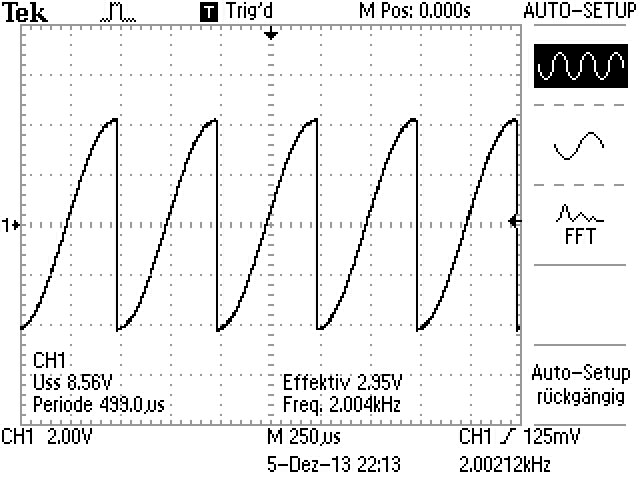
\includegraphics[scale=0.85]{Bilder/5-sine-270.png}
\caption{Output des Mischers bei unverrauschtem Signal ($\Delta\phi=270^\circ$)}
\label{Abb10}
\end{figure}


\begin{figure}[h]
\centering
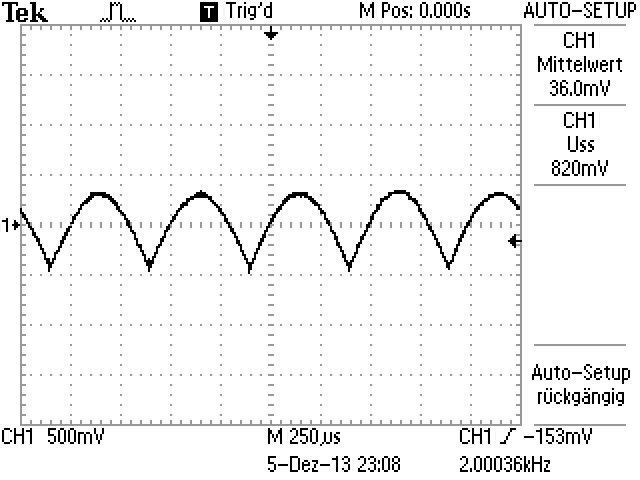
\includegraphics[scale=0.85]{Bilder/5-noise-0.png}
\caption{Output des Mischers bei verrauschtem Signal ($\Delta\phi=0^\circ$)}
\label{Abb11}
\end{figure}

\begin{figure}[h]
\centering
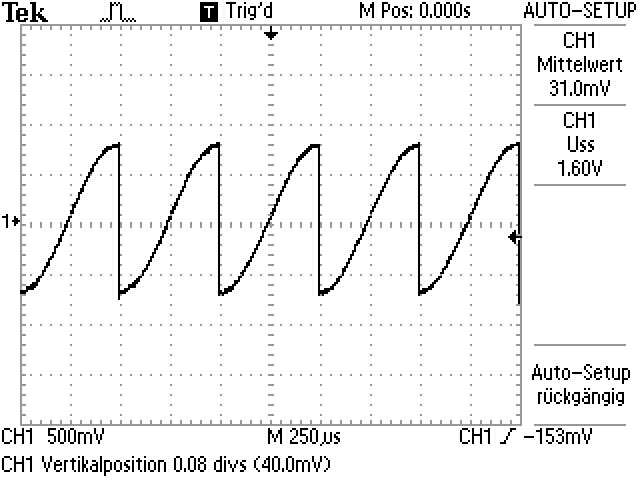
\includegraphics[scale=0.85]{Bilder/5-noise-90.png}
\caption{Output des Mischers bei verrauschtem Signal ($\Delta\phi=90^\circ$)}
\label{Abb12}
\end{figure}

\begin{figure}[h]
\centering
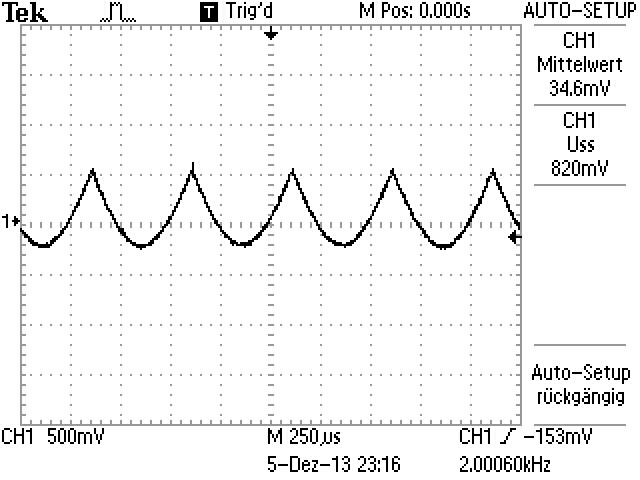
\includegraphics[scale=0.85]{Bilder/5-noise-180.png}
\caption{Output des Mischers bei verrauschtem Signal ($\Delta\phi=180^\circ$) }
\label{Abb13}
\end{figure}

\begin{figure}[h]
\centering
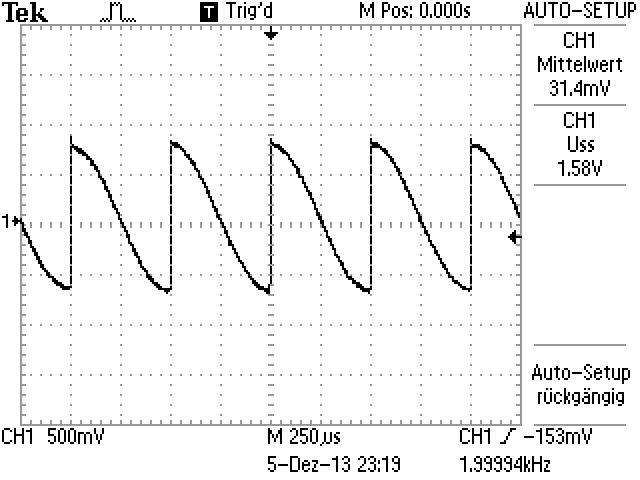
\includegraphics[scale=0.85]{Bilder/5-noise-270.png}
\caption{Output des Mischers bei verrauschtem Signal ($\Delta\phi=270^\circ$)}
\label{Abb14}
\end{figure}



\end{document}
